\section{The Rust Model}
\thispagestyle{plain} % surpress header on first page

This section follows up on the previous one in the sense that it introduces the model created by \cite{Rust.1987} and presents how NFXP and MPEC can be used to estimate its model parameters. My notation is mainly inspired by the one employed in \cite{Su.Judd.2012}. 

\subsection{The Economic Model}

Rust's model is based on the decision making process of Harold Zurcher who is in charge of a bus fleet and has to decide in each period $t = 0, 1, 2, ...$ whether to replace the engine ($d^i_t=1$) of one or more buses $i = 1, 2, ..., M$ in his fleet or otherwise repair them in a less costly way ($d^i_t=0$). The agent, hence, chooses from the action space $\mathcal{D} = \{0, 1\}$. He bases this choice on two state variables which are the observed cumulative mileage $x^i_t$ of a bus since the last engine replacement and some unobserved (by the econometrician) factor $\epsilon^i_t$. The state of a bus $i$ in period $t$ is therefore fully described by ($x^i_t$, $\epsilon^i_t$) $\in \mathcal{S}$. The agent receives an immediate reward in period $t$ from the chosen replacement decision $d^i_t(x^i_t, \epsilon^i_t)$. The choice in turn affects the possible state space $\mathcal{S'}$ in the period $t+1$ as the cumulative mileage after replacement $x^i_{t+1}$ depends on the choice of $d^i_t$. As the agent is forward looking with a discount factor $\beta \in (0, 1)$ he does not simply maximize the immediate reward but rather the expected discounted utility over an infinite horizon with a higher preference for reward occurring closer to the present. The immediate reward can be characterized in the following way: 

\begin{equation}
	u(x^i_t, d^i_t, \epsilon^i_t; \theta_1, RC) = v(x^i_t, d^i_t; \theta_1, RC) + \epsilon^i_t
\end{equation}

with 

\[v(x^i_t, d^i_t; \theta_1, RC) = \left\{
\begin{array}{lr}
-c(x; \theta_1)  & \mbox{if } d^i_t = 0 \\
-RC -c(0;\theta_1) & \mbox{if } d^i_t = 1
\end{array}
\right.
\]

The immediate reward is hence determined by some operating cost $c(.)$ if regular maintenance as opposed to engine replacement is chosen. It consists of a replacement cost $RC$ and the operating cost after resetting the cumulative mileage to zero if replacement is picked. This shows that The choice of the agent $d^i_t$ depends crucially on the cost parameters $\theta_1$ and $RC$. The timing of events for a single bus in the decision process of Harold Zurcher is depicted in Figure \ref{Figure1} below. 
\vspace{2ex}

\begin{figure}[H]
	\caption{\label{Figure1}Timing of the Decision Model}
	\vspace{2ex}
	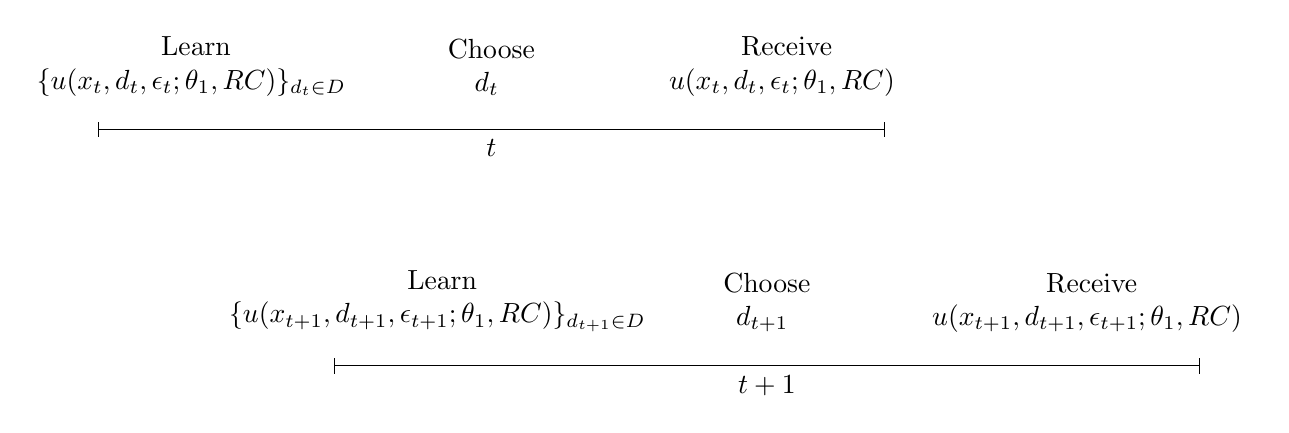
\begin{tikzpicture}
	\draw [|-|]
	(0,1) -- (10,1)
	node [above,align=center,very near start]
	{
		Learn\\
		$\{u(x_t, d_t, \epsilon_t; \theta_1, RC)\}_{d_t \in D}$
		\vspace{2ex}
	}
	node [above,align=center,midway]
	{
		Choose\\
		$d_t$
		\vspace{2ex}
	}
	node [above,align=center,very near end]
	{
		Receive\\
		$u(x_t, d_t, \epsilon_t; \theta_1, RC)$
		\vspace{2ex}
	}
	node [below, align=center, midway]
	{$t$};
	\draw [|-|]
	(3,-2) -- (14,-2)
	node [above,align=center,very near start]
	{
		Learn\\
		$\{u(x_{t+1}, d_{t+1}, \epsilon_{t+1}; \theta_1, RC)\}_{d_{t+1} \in D}$
		\vspace{2ex}
	}
	node [above,align=center,midway]
	{
		Choose\\
		$d_{t+1}$
		\vspace{2ex}
	}
	node [above,align=center,very near end]
	{
		Receive\\
		$u(x_{t+1}, d_{t+1}, \epsilon_{t+1}; \theta_1, RC)$
		\vspace{2ex}
	}
	node [below, align=center, midway]
	{$t+1$};
	
	\end{tikzpicture}
\end{figure}


The transition of the state vector ($x^i_t$, $\epsilon^i_t$) is assumed to follow a Markov process, i.e. the current state only depends on the previous one and hence the utility maximization problem is time-invariant. Dropping the bus index $i$ for convenience, the optimization problem of the agent gives rise to the following value function for a single bus: 

\begin{equation}
V(x_t, \epsilon_t) = \max_{\{d_t, d_{t+1}, ... \}} \E \left[\sum_{\tau=t}^{\infty} \beta^{\tau - t} u(x_\tau, d_\tau, \epsilon_\tau; \theta_1, RC)\right]
\end{equation}

Solving this model leads to an optimal policy rule $\pi^* = (d^{\pi^*}_t(x_t, \epsilon_t))^\infty_t$.

\subsection{The Model Solving}
Given some simplifying assumptions such as conditional independence on the transition probabilities of the state vector, the assumption that the error term $\epsilon_t$ follows a multivariate extreme-value distribution and after discretizing the possible values of the state variable $x$, Rust derives the following fixed point equation needed to solve the economic model:

\begin{equation}
	\label{eq5}
	EV(\hat x_k, d) = \sum_{j=0}^{J} log \left\{ \sum_{d'\in\{0, 1\}}  exp[v(x', d'; \theta_1, RC) + \beta EV(x', d')]\right\} \times p_3(x'|\hat x_k, d; \theta_3). 
\end{equation}

with

\[p_3(x'|\hat x_k, d; \theta_3) = \left\{
\begin{array}{lr}
	Pr\{x'=\hat x_{k+j}|\theta_3\}  & \mbox{if } d = 0 \\
	Pr\{x'=\hat x_{1+j}|\theta_3\} & \mbox{if } d = 1
\end{array}
\right.
\]

for $j=0, 1, ..., J$ indicating how many grid points the mileage state climbs up in the next period. \paragraph{}

In the above equation $\hat x_k$ represents the grid point $k$ of the state variable $x$ while $\hat x_1 = 0$. The number of possible $\hat x_k$ depends on the choice of the grid size $K$ set by the researcher. All the variables $v$ depict current period variables while variables $v'$ display the value in the next period. The probability $p_3$ indicates how likely it is that a bus moves up a specific amount of grid points in the next period depending on the structural parameter $\theta_3$. Imagine now we decide to set the grid size to $K=90$ as done by \cite{Rust.1987}, then we generally have to find the fixed point above which yields $EV = [EV(\hat x_1, 0), ..., EV(\hat x_{90}, 0), EV(\hat x_1, 1), ..., EV(\hat x_{90}, 1)]$. This simplifies, though, as all the expected values from $EV(\hat x_1, 1), ..., EV(\hat x_{90}, 1)$ are actually equivalent to $EV(\hat x_1, 0)$. This means that in our scenario we just have to find the fixed point for $d=0$, i.e. in our example the vector $EV$ has a dimension of $90$. This observation will later be important for the difference between NFXP and MPEC. \cite{Su.Judd.2012} denote the simplified version of equation \ref{eq5} shorthand as:

\begin{equation}
	EV = T(EV, \theta)
\end{equation}

The solution to this fixed point can now be used to derive conditional choice probabilities of the agent: 

\begin{equation}
	P(d|\hat x; \theta) = \frac{exp[v(\hat x, d; \theta_1, RC) + \beta EV(\hat x, d)]}{\sum_{d' \in \{0, 1\}} exp[v(\hat x, d'; \theta_1, RC) + \beta EV(\hat x, d')]}.
\end{equation}

The above equation describes the probability that the agent chooses $d$ given that the observed mileage state is at a certain grid point $\hat x$. This derivation depends on both the cost parameters ($\theta_1$, $RC$) directly and indirectly through $EV(.)$ on the transition parameter $\theta_3$. These conditional choice probabilities together with the transition probabilities $p_3(.)$ become relevant in the next section when calibrating the model using maximum likelihood. 


\subsection{Calibration}

Describe NFXP and MPEC in the context of the Rust model and write some pseudo code again.
